\documentclass[onecolumn, 12pt]{article}

%!TeX spellcheck = en-US,fr
  \usepackage[utf8]{inputenc}
  \usepackage{hyperref}
  \usepackage[T1]{fontenc}
  \usepackage[francais]{babel}
  \usepackage{layout}
  \usepackage{verbatim}[4]
  \usepackage{color}

  \usepackage{graphicx}
  \usepackage{caption}


  \usepackage{titlesec}

  \setcounter{secnumdepth}{4}

  \titleformat{\paragraph}
  {\normalfont\normalsize\bfseries}{\theparagraph}{1em}{}
  \titlespacing*{\paragraph}
  {0pt}{3.25ex plus 1ex minus .2ex}{1.5ex plus .2ex}


  \title{État de l'art sur la \textit{Stance Detection}.}
  \author{Enzo Poggio}
\begin{document}
\maketitle{}
\begin{abstract}
 Dans cette partie nous allons présenter la \textit{Stance Detection} et lui donner une définition rigoureuse.
 Nous discuterons les différentes tâches partagées qui ont eu lieu autour de la \textit{Stance Detection}. Notamment nous présenterons les corpus et les méthodes de classification choisies.
\end{abstract}

\section{Vers une définition.}
\subsection{Formalisation de la \textit{Stance Detection}.}
La \textit{Stance Detection} ou en français la détection de parti pris
\footnote{Vous remarquerez que pour la cohérence et pour la consistance de ce document nous  n'emploierons plus que la formulation \og détection de parti pris\fg au lieu de \og\textit{Stance Detection}\fg.}
est la méthode qui permet de déterminer si un énoncé \textbf{E} par rapport à une cible \textbf{C} donnée est en accord ou en désaccord avec la cible.
On l'utilise aussi parfois pour déterminer si l'énoncé discute sans parti pris de la cible.
C'est-à-dire que \textbf{E} parle de \textbf{C} mais on ne trouve aucun indice soit en faveur, soit en défaveur la cible.
Par extension, si on arrive à déterminer la cible, on peut connaître les énoncés qui n'y correspondent pas.
Ce type d'énoncé indépendant ne donne aucun indice de prise de parti et surtout aucun indice de la cible en général.
La cible et l'énoncé ne partagent aucun lien direct ou indirect.
Ainsi la détection de parti pris nous permet de repérer ces quatre cas de figure:

\begin{description}
 \item [E est pour C] quand l'énoncé montre un ou des indices en faveur de la cible.
 \item [E est contre C] quand l'énoncé montre un ou des indices en contradiction avec la cible.
 \item [E discute C] quand l'énoncé donne une ou des informations sur la cible sans donner d'indices de parti pris comme dans les deux cas pécédents.
 \item [E est non-lié à C] quand l'énoncé ne donne aucune information par rapport à la cible en général.
\end{description}

Les deux derniers cas ne détectent aucun parti pris.
Mais ils restent pertinents pour la détection de parti pris doit intégrer une limitation à un sujet donné.
Une telle détection implémente donc un module de détection des relations.
Appellons \textbf{R} la relation entre \textbf{E} et \textbf{C}.


\subsection{Domaine de la détection de parti.}
Nous avons beaucoup parlé d'indices dans la partie précédente.
Questionnons leur nature.
La détection de parti pris se base sur la relation entre la cible et l'énoncé.
La nature de cette relation est sémantique.
Les traits qui permettent d'unir l'énoncé et la cible pour déterminer le parti pris doivent alors aussi entretenir une relation sémantique.
On verra plus tard que certaines relations syntaxiques peuvent être utiles de manière localisées dans certaines tâches.

Il apparait un problème dû à la sémantique: il faut s'accorder au préalable sur le sens des mots et sur ce que désignent nos cibles et leurs rapports avec l'énoncé.
En effet, pour constituer un corpus de prise de position par rapport à un énoncé, il faudra trouver la manière la plus objective de qualifier la relation entre l'énoncé et la cible.
\subsection{La genèse de la détection de parti pris.}

Une des premières publications sur la déctection de prise de parti était \og  \textit{Cats Rule and Dogs Drool![...]} \fg (voir \href{http://www.aclweb.org/anthology/W11-1701}{Pranav Anand et al, 2011}) qui cherchait à classer la prise de position dans des débats en ligne sur des sujets variés.
Leur but était de montrer que les débats idéologiques comportent une plus grande part de messages de réfutation.
La publication montrait aussi qu'il est beaucoup plus difficile de classer les posts de réfutation, aussi bien pour les humains que pour les classificateurs automatiques formés à la détection de prise de parti.

Les chercheurs ont créé leur corpus à partir de 1113 débats bi-partiaux (soit 4873 posts) dans 14 sujets différents du site \href{http://www.convinceme.net/}{ConvinceMe.net}.
Pour annoter le corpus, les chercheurs ont demandé à neuf participants de mettre une étiquette sur différentes parties de débat sur le site.
Il est intéressant de notifier que les annotateurs  n'ont eu que 0.73 d'exactitude croisée dans la classification des réfutations (tous sujets confondus).
Ainsi le problème sémantique est réel.
Les annotateurs ne tombent pas d'accord sur la relation sémantique de certains énoncés par rapport à leurs cibles.
Le but d'un système automatique de classification des réfutations sera donc de s'approcher au plus de ce pourcentage d'exactitude pour représenter au mieux le classement humain général.

L'équipe d'Anand a fait plusieurs modèles de système utilisant des traits différents (n-grams, la ponctuation répétée, LIWC, dépendance syntaxique,...).
Ces modèles utilisaient soit une implémentation de Naive Bayes, soit une implémentation de JRip\footnote{JRip est un classificateur basé sur des règles qui produisent un modèle compact adapté à la conception d'application rapide.} en fonction des traits choisis.

Les résultats des modèles varient en fonction des sujets entre 0.59 et 0.69 d'exactitude pour la détection de réfutation.
De plus, aucun modèle ne se départage des autres.
Tous ont plus ou moins réussi selon un sujet différent.
La moyenne est 0.63 pour la détection de réfutation.
C'est dix points de moins que l'exactitude humaine (qui varie entre 0.66 et 0.94).

Premièrement, cette publication nous montre combien il est ardu de se confronter à la sémantique.
En droit, le sens d'un énoncé devrait être univoque et susciter une seule relation universelle entre la cible et l'énoncé.
En fait, nous -les annotateurs humains- sommes tous soumis à des biais, des opinions, des préjugés qui ne permettent qu'un recouvrement subjectif de la relation entre cible et énoncé.

Deuxièmement, ce papier montre la difficulté de la tâche.
Aucun modèle possédant des traits particuliers n'a eu de meilleur résultat dans tous les sujets confondus.

Nous avons présenté un des premiers travaux sur la détection de parti pris.
Par la suite, nous nous limiterons à des travaux plus récents.
Ceux-ci s'intéressent à notre sujet: les \textit{Fake News}.

\subsection{Application générale et relative au \textit{Fake News}.}
Nous allons voir dans les sections suivantes les différentes utilisations de la détection de parti pris à travers deux tâches partagées.
Premièrement dans la section \no2, nous verrons l'utilisation de la détection de parti pris à l'intérieur de \textit{tweets} sur des sujets polémiques; grâce à la \textbf{\textit{SemEval-2016 Task 6}}.
Puis deuxièmement dans la section \no3, nous verrons l'utilisation de la détection de parti pris pour la détection de \textit{Fake News} ; grâce au \textbf{\textit{Fake News Challenge}}.
Nous proposerons dans la troisième partie de ce mémoire une contribution originale de la tâche que nous discutons dans la section \no3.



%%%%%%%%%%%%%%%%%%%%%%%%%%%%%%%%%%%%%%%%%%%%%%%%%%%%%%%%%%%%%%%%%%%%%%%%%%%%%%%
%%%%%%%%%%%%%SemEval-2016 Task 6%%%%%%%%%%%%%%%%%%%%%%%%%%%%%%%%%%%%%%%%%%%
%%%%%%%%%%%%%%%%%%%%%%%%%%%%%%%%%%%%%%%%%%%%%%%%%%%%%%%%%%%%%%%%%%%%%%%%%%%%

\section{\textit{SemEval-2016 Task 6}.}
\subsection{Description générale de la tâche.}
Cette tâche porte le nom de \og \textit{Detecting Stance in Tweets} \fg (\href{https://www.aclweb.org/anthology/S/S16/S16-1003.pdf}{Saif M.
Mohammad et al, 2016}).
Le but de la tâche est de déterminer la relation \textbf{R} entre un tweet \textbf{E} et une cible \textbf{C}.

Ici, nous avons trois classes possibles pour déterminer le parti du tweeter par rapport à son tweet:
\begin{description}
 \item [favor] s'il est en faveur la cible.
 \item [against] s'il est contre la cible
 \item [neither] si il n'est ni en faveur la cible, ni il n'est contre la cible.
\end{description}

Exemple direct:

\begin{description}
 \item [C] Hillary Clinton
 \item [E] Hillary Clinton has some strengths and some weaknesses.
 \item [R] neither
\end{description}

Exemple indirect:
\begin{description}
 \item [C] legalization of abortion
 \item [E] A foetus has rights too! Make your voice heard.
 \item [R] against
\end{description}

\newpage
La tâche se divise en deux sous-tâches:
% la première \textbf{A} supervisée et la deuxième \textbf{B} non-supervisée.

\subsubsection{Sous-tâche A.}
La sous-tache A est supervisée.
Elle porte sur cinq différents sujets (\textit{‘Atheism’},\textit{ ‘Climate Change is a Real Concern’},\textit{‘Feminist Movement’}, \textit{‘Hillary Clinton’},\textit{‘Legalization of Abortion’}).
Elle contient 4163 couples \textbf{C/E} labélisés \textbf{R}.
On réserve 30\% pour l'ensemble de test et le reste pour l'ensemble d'entraînement.

\subsubsection{Sous-tâche B.}
La sous-tache B est non-supervisée.
Elle porte sur un seul thème (\textit{‘Donald Trump’}).
L'ensemble test est constitué de 707 tweets \textbf{E}.
Aucun ensemble d'entraînement n'a été donné.
Mais un ensemble de 78 000 tweets non-labélisés à propos de Donald Trump était disponible.

\subsubsection{Évaluation.}
Pour l'évaluation des systèmes on utilise le F1-score moyen; calculé ainsi:
\begin{equation}
 F_{avg} = \frac{F_{favor}+F_{against}}{2}
\end{equation}
Avec F$_{favor}$  et F$_{against}$ ainsi calculés:

\begin{equation}
 F_{favor} = \frac{2P_{favor}R_{favor}}{P_{favor}+R_{favor}}
\end{equation}
\begin{equation}
 F_{against} = \frac{2P_{against}R_{against}}{P_{against}+R_{against}}
\end{equation}
\subsection{Les participants.}
Il y a eu 19 dépots pour la sous-tâche A et 9 dépots pour la sous-tâche B.
Premièrement, nous parlerons de la réussite à la tâche en général.
Deuxièment, nous discuterons seulement de quelques dépots intéressantes.
Et troisièment, nous comparerons les différents protocoles vus.

\subsubsection{Dépots en général.}
Parmi les 19 dépots de la sous-tâche A aucun système n'a dépassé les baselines.
En effet, Saif M.
Mohammad et al ont fourni 4 baselines pour la sous-tâche A.
La première baseline naïve donnait le label majoritaire à toutes les entrées (\textit{Majority class}).
Les trois suivantes utilisent un ou plusieurs classificateurs linéaires (SVM) pour labéliser les entrées.
La deuxième utilisent 5 classificateurs SVM (un pour chaque différent sujet) sur les vecteurs d'unigrams de la combinaison de \textbf{C} et \textbf{E} (\textit{SVM-unigrams}).
De la même manière la troisième a aussi 5 SVM mais utilise comme dimensions de vecteur :
les 1-2-3-grams pour les mots et les 2-3-4-5-grams pour les caractères (\textit{SVM-ngrams}).
Et pour finir, la quatrième baseline utilise un seul SVM sur les mêmes dimensions de vecteur que la troisième baseline (\textit{SVM-ngrams-comb}).

En revanche, 7 des 9 équipes ont réussit à battre les baselines de la sous-tâche sur B.
Ces baselines reprennent certaines baselines de la sous-tâche A à savoir la première  \textit{Majority class} et la quatrième \textit{SVM-ngrams-comb}.

Pour la sous-tâche A, la plupart des équipes ont utilisé des fonctions de classification de texte standard tels que n-gram et vecteurs de mots, des lexiques de sentiments.
Certaines équipes ont interrogé Twitter sur des hashtags, pour marquer des prises de parti plus déterminantes.
Certaines ont entrainé leurs systèmes à partir de  vecteurs de Google Actualitée ou directement des corpus Twitter.

Et pour la sous-tâche B, certaines équipes ont très bien détecté les tweets en faveur
de Trump. Grâce aux tweets qui se trouvaient dans le corpus de Clinton en inversant leur valeur.

\subsubsection{Dépots particuliers.}
Ici, de manière succinte, nous allons décrire les différents modèles des meilleurs systèmes pour les différentes tâches.

\paragraph{MITRE 1er pour la tâche A.}

\begin{center}
 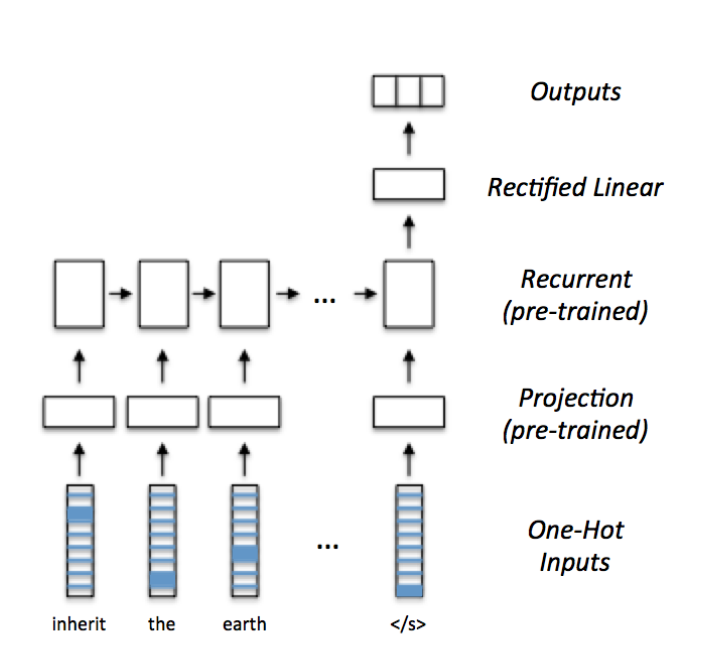
\includegraphics[scale=0.25]{../../img/model/mitre/model.png}
 \captionof{figure}{Le réseau neuronal récurrent de MITRE pour la détection de parti pris.}
 \label{mitre_model}
\end{center}

L'approche de détection de prise de parti de MITRE utilise un réseau de neurones récurrent organisé en quatre couches de poids.
Chaque mots est projeté comme une entrée dans une couche d'\textit{embbeding} de 256 dimensions (créé avec word2vec), qui alimente en une couche récurrente contenant 128 LSTM.
La sortie du terminal
de cette couche récurrente est densément connecté à un 128 classifieurs linéaires
Cette même couche est entièrement connectée à un softmax tri-dimentionnel dans laquelle chaque unité représente l'une des classes de sortie: FAVOR, AGAINST ou NONE.

\paragraph{pkudblab 2ème pour la tâche A.}
\begin{center}
 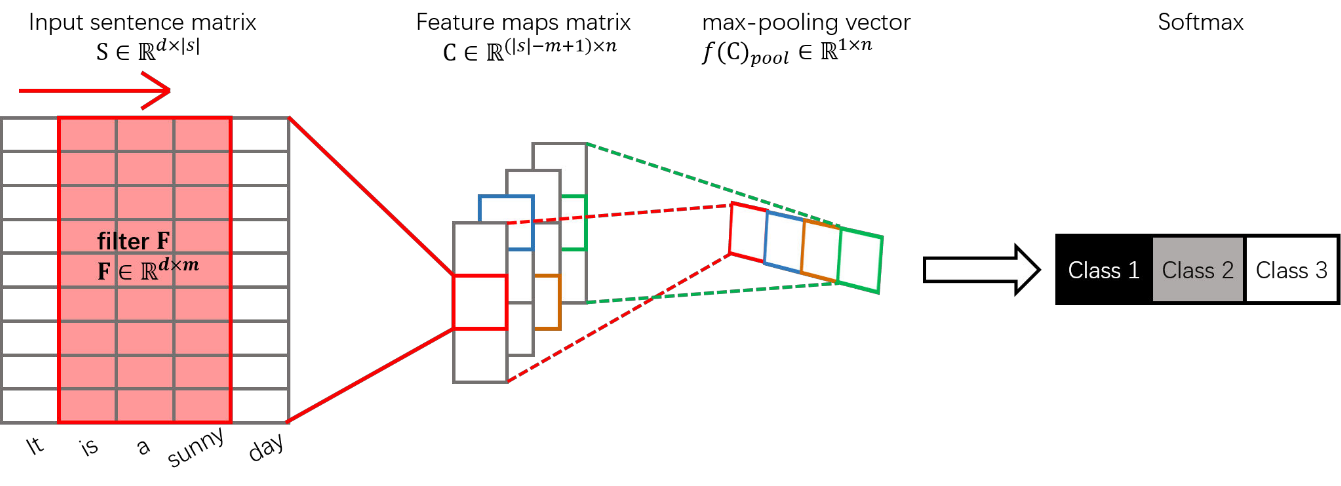
\includegraphics[scale=0.25]{../../img/model/pkudblab/model.png}
 \captionof{figure}{Architecture principale du réseau de neurones convolutionnels de pkudblab.}
 \label{pkudblab_model}
\end{center}
L'Architecture principale de pkudblab est un réseau de neurones convolutionnels.
On peut en décrire 5 composant majeurs:
\begin{description}
 \item[Une table de correspondance] est une énorme matrice d'embbeding de mots.
 Chaque colonne de la table, correspond à un mot.
 Chaque mot incorporé dans cette table a été pré-formé par des vecteurs de word2vec (Mikolov et al., 2013).
 Ces vecteurs sont formés sur une partie de l'ensemble de données Google News.
 \item[Une matrice d'entrée] représente d'une phrase d'entrée et la longueur de la phrase.
 \item[La couche convolution] a pour but d'extraire des paternes, de sorte que certaines formulations abstraites communnes soient représentées.
 \item[Le Pooling layer] a pour but est de simplifier l'information dans le
 sortie de la couche convolutionnelle.
 \item[La Couche de sortie softmax] est entièrement connectée et est destinée à la classification.
\end{description}

Pour la sous-tâche A, ils ont séparées les ensembles de données en cinq sous-ensembles.
Ils ont donc entrainé de manière séparé les modèles sur les différents sujets.

\paragraph{pkudblab 1er pour la tâche B.}

Pour la sous-tâche B, ils ont utilisé le même modèle que pour A.
Pour entraîner leur modèle ils établissent un ensemble de données de formation à deux classes (favor, against) à partir du corpus du domaine officiel en fonction de plusieurs expressions spéciales.

\subsubsection{Discussions comparatives.}
% tableau rérésultats tâches A
\begin{center}
 \begin{tabular}{| c | c | c || c |}
  \hline
  \textbf{Baseline} & \textbf{F$_{favor}$} & \textbf{F$_{against}$} & \textbf{F$_{avg}$} \\
  \hline
  Majority class    & 52.01                & 78.44                  & 65.22              \\
  SVM-unigrams      & 54.49                & 72.13                  & 63.31              \\
  SVM-ngrams        & 62.98                & 74.98                  & 68.98              \\
  SVM-ngrams-comb   & 54.11                & 70.01                  & 62.06              \\
  \hline
  \textbf{Équipe}  &                      &                        &                    \\
  \hline
  MITRE             & 59.32                & 76.33                  & 67.82              \\
  pkudblab          & 61.98                & 72.67                  & 67.33              \\
  TakeLab           & 60.93                & 72.67                  & 66.83              \\
  \hline
 \end{tabular}
 \captionof{table}{Résultats pour la sous-tâche A des baselines et des 3 premiers participants ordonnés.}
\end{center}


% commentaires
On voit qu'il est difficile de faire décoller les scores mêmes avec les meilleurs systèmes.
Ceci nous donne une bonne idée de l'état de l'art en 2016.
Une implémentation simple avec des n-grams bien choisis et une catégorisation aident beaucoup à avoir de bons résultats.
Mais est-ce toujours possible de contextualiser les données ? Il y a un biais notoire du fait de  travailler avec une micro vocabulaire en plus souvent réduit sémantiquement par l'algorithme.
% tableau tâches B
\begin{center}
 \begin{tabular}{| c | c | c || c |}
  \hline
  \textbf{Baseline} & \textbf{F$_{favor}$} & \textbf{F$_{against}$} & \textbf{F$_{avg}$} \\
  \hline
  Majority class    & 0.00                 & 59.44                  & 29.72              \\
  SVM-ngrams-comb   & 18.42                & 38.45                  & 28.43              \\
  \hline
  \textbf{Équipe}  &                      &                        &                    \\
  \hline
  pkudblab          & 57.39                & 55.17                  & 56.28              \\
  LitisMind         & 30.04                & 59.28                  & 44.66              \\
  INF-UFRGS         & 32.56                & 52.09                  & 42.32              \\
  \hline
 \end{tabular}
 \captionof{table}{Résultats pour la sous-tâche B des baselines et 3 premiers participants ordonnés.}
\end{center}

La tâche dîte non-supervisée a fini par l'être.
Au final les équipes ont utilisé le corpus d'Hillary Clinton pour former celui de Trump.
Ils ont juste ajouté quelques expressions clichés trouvé la faveur ou la défaveur du tweet.
Le sujet de cette sous-tâche est particuliérement clivant.
Cela ne permet pas de retirer une méthode d'apprentissage non supervisé objective.

%%%%%%%%%%%%%%%%%%%%%%%%%%%%%%%%%%%%%%%%%%%%%%%%%%%%%%%%%%%%%%%%%%%%%%%%%%%%%%%%
%%%%%%%%%%%%%%%%FNC%%%%%%%%%%%%%%%%%%%%%%%%%%%%%%%%%%%%%%%%%%%%%%%%%%%%%%%%%%%%%
%%%%%%%%%%%%%%%%%%%%%%%%%%%%%%%%%%%%%%%%%%%%%%%%%%%%%%%%%%%%%%%%%%%%%%%%%%%%%%%%

\section{\textit{Fake News Challenge}.}

\subsection{Description générale de la tâche}
Nous présentons dans cette section la tâche partagée qu'est le \textit{Fake News Challenge} et les différentes solutions proposées par ses participants.
Pour détecter des \textit{Fake News} il nous faut résoudre plusieurs défis à savoir:
\begin{enumerate}
 \item Déterminer si les faits présents dans l'article de presse sont corrects; c'est-à-dire déterminer la véracité des faits par rapport au monde réel.
 \item Analyser les relations entre le titre de l'article et le corps de l'article.
 \item Quantifier le biais inhérent d'un texte.
\end{enumerate}
On voit clairement une application de la détection de parti pris dans le défi \no2.
En effet ce défi correspond parfaitement à sa définition.

Évaluer la véracité d'un article est une tâche complexe et lourde, même pour des experts formés.
La première étape du Fake News Challenge se concentre sur la tâche de détection de parti pris.
\subsubsection{But.}
L'objectif du Fake News Challenge est d'explorer comment les technologies
d'intelligence artificielle pourraient être utilisées pour lutter contre les
fake news.
\subsubsection{Organisation générale.}
Vous pouvez retouver toutes les infomations du \href{http://www.fakenewschallenge.org/}{Fake News Challenge} sur leur site officiel.
Et vous pouvez retrouver les codes de leur \href{https://github.com/FakeNewsChallenge/fnc-1-baseline}{baseline} et \href{https://github.com/FakeNewsChallenge/fnc-1}{les données} sur github.


\subsubsection{Données et origines des données.}
Le FNC est une tâche partagée supervisée.
Les donneés sont pourvues par les organisateurs.
Ils définissent les données en termes d'entrées et de sorties.Une entrée est le couple formé par une affirmation \textbf{C} et un corps de texte \textbf{E}; soit à partir du même article de nouvelles ou de deux articles différents.
Une sortie est la relation \textbf{R} corps du texte par rapport à la revendication faite dans l'affirmation définie par l'une de ces quatre catégories:

\begin{description}
 \item [related:] Le corps du texte \textbf{E} et l'affirmation \textbf{C} traitent d'un sujet en commun\footnote{Cette méta-relation ne labélisera jamais les données elle est là pour mieux comprendre le but de la détection de prise de parti.}.
 \begin{description}
  \item [agree:] Le corps du texte \textbf{E} est en accord avec l'affirmation \textbf{C}.
  \item [disagree:] Le corps du texte \textbf{E} n'est pas d'accord avec l'affirmation \textbf{C}.
  \item [discuss:] Le corps du texte discute \textbf{E} le même sujet que l'affirmation \textbf{C}, mais ne prend pas de parti pris.
 \end{description}
 \item [unrelated:] Le corps du texte \textbf{E} traite d'un sujet différent de l'affirmation \textbf{C}.
\end{description}

\href{http://aclweb.org/anthology/N/N16/N16-1138.pdf}{Ferreira \& Vlachos (2016)} ont au préalable testé et créé un ensemble de donneés à partir du \href{http://www.emergent.info/}{site du projet Emergent} de Craig Silverman.
Le projet Emergent fut aussi utile pour la création du corpus de la FNC.

Les données de ce projet ont été collectées par des journalistes du \href{https://towcenter.org/}{\textit{Tow Center for Digital Journalism}}.
Pour ajouter une entrée au site, le journaliste doit trouver deux choses: une affirmation qui semble être une rumeur et un ensemble d'articles qui parlent de cette soi-disant rumeur.
Les sujets de chaque affirmation varient, cela va des dixits politiques de Donald Trump aux comparaisons de prix de la prochaine Apple Watch.
Les sources de celles-ci sont les comptes twitter polémiques, traitant les rumeurs et les sites tel que Snopes.com\footnote{\href{https://www.snopes.com/}{Snopes.com} est un site Web anglophone créé dans le but de limiter la propagation des canulars informatiques et des rumeurs infondées circulant sur Internet.}.À partir de certaines affirmations, le journaliste constitue donc un corpus d'articles pour établir la véracité de celles-ci.
Donc chaque affirmation peut être \og Vraie\fg, \og Fausse\fg ou \og Non-vérifié\fg.
Cette valeur de vérité peut être établie grâce au corpus d'articles; où chaque article peut soit être \og Pour\fg, \og Contre\fg ou \og Neutre\fg.
Le journaliste résume l'article en un gros titre (\textit{headline} à ne pas confondre avec notre affirmations de rumeurs).
Ce n'est pas le nombre d'articles \og Pour\fg  ou \og Contre\fg la véracité des affirmations; mais bien sur la vraissemblance des preuves qui sont rapportées dans les articles jugées par le journaliste.

Le corpus de Ferreira \& Vlachos est composé alors de 300 affirmations de rumeurs dont 2595 articles sont associés à un ratio de 8,75 articles pour une affirmation.
La distribution hétérogène  est de 47.7\% \og Pour\fg, 15.2\% \og Contre\fg et 37.1\% \og Neutre\fg.
Pour tester si les données d'Emergent étaient assez discriminatives et robustes pour une tâche d'apprentissage automatique, Ferreira \& Vlachos ont testé l'accord entre les gros titre des journalistes et les affirmations de rumeurs.
Nous ne détaillerons pas plus leur protocole ici.
Mais leur 73\% d'exactitude (par rapport aux 47\% de leur baseline naïve) donne une bonne estimation de la consistance des données.

La répartitions des donneés de la FNC est faite avec le même procédé mais cette fois-ci on est extrait l'affirmation de rumeurs et le corps des articles.
De plus les organisateurs ajoutent une dimension de classification; la classe \textbf{unrelated}  est formée à partir des couples affirmation et de valeurs qui n'ont pas de liens sur la plateforme Emergent.
Les sujets sont alors non-liés.
La répartition des données au niveau des relations \textbf{R} se fait donc ainsi pour l'entrainement: 73.13\% sont \textbf{unrelated}, 17.82\% sont \textbf{discuss}, 7.36\% sont \textbf{agree} et 1.68\% sont \textbf{disagree}.
En chiffre cela donne 37727 corps d'articles \textbf{E} pour 1648 affirmations de rumeurs \textbf{C}.
Ce qui a donné 49973 couples \textbf{C/E}.
L'ensemble de test est composé de 20019 corps d'articles \textbf{E}, 894 affirmations de rumeurs \textbf{C} et donc de 25419 couples \textbf{C/E}.
Bien sûr, les données \textbf{E} ou \textbf{C} entre le test et l'entrainement ne se recoupent pas et les relations \textbf{R} ne sont pas données dans le test.

Voici un exemple de données pour l'affirmation \textbf{C} suivante \og \textit{Robert Plant Ripped up \$800M Led Zeppelin Reunion Contract} \fg:

\begin{description}
 \item [R: Agree] \textbf{E}: \og \textit{ … Led Zeppelin’s Robert Plant turned down £500 MILLION to reform supergroup.
  … } \fg
 \item [R: Disagree] \textbf{E}: \og \textit{ … No, Robert Plant did not rip up an \$800 million deal to get Led Zeppelin back together.
  … } \fg
 \item [R: Discusses] \textbf{E}: \og \textit{ … Robert Plant reportedly tore up an \$800 million Led Zeppelin reunion deal.
  … } \fg
 \item [R: Unrelated] \textbf{E}: \og \textit{ … Richard Branson’s Virgin Galactic is set to launch SpaceShipTwo today.
  …} \fg
\end{description}



\subsubsection{L'évaluation.}
\begin{center}
 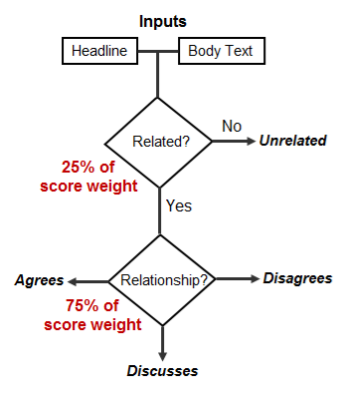
\includegraphics[scale=0.5]{../../img/fnc-eval/fnc-eval.png}
 \captionof{figure}{Diagramme de calcul du score relatif.
  Traduire ici \og Headline\fg par \textbf{C} et  \og Body Text\fg par \textbf{E}.}
 \label{fig_eval}
\end{center}

Les équipes seront évaluées selon un système de score relatif pondéré à deux niveaux; pour le premier niveau il faut classer \textbf{E} et \textbf{C} comme étant liés ou non (25\% de la pondération).
Puis pour le deuxième niveau il faut classer les couples liés comme étant d'accord, en désaccord ou discuté (75\% de la pondération), trouver le bon \textbf{R} du couple.
Le score relatif est le score brut normalisé par le score maximum possible sur l'ensemble de test \footnote{Nous donnerons à chaque fois le score brut et le score normalisé en pourcent.}.
En effet, il est très facile d'avoir une très bonne exactitude avec une classe sur-représentée comme les \textbf{unrelated} (73.13\% du corpus d'entrainement).
Il y a donc deux règles qui régissent ce score:
\begin{description}
 \item [unrelated/related :] si la classe Gold et la classe attiribué ont la même méta-classe alors on ajoute 0.25 au score.
 \item [same related :] si entre deux classe \textbf{related} la classe Gold et la classe attiribuée sont les mêmes, alors on ajoute 0.75 au score.
\end{description}

Exemples de scores en fonction de l'attribution de classe:

\begin{center}
 \begin{tabular}{| c | c || l | }
  \hline
  \textbf{Classe Gold} & \textbf{Classe attribuée} & \textbf{Score} \\
  \hline
  unrelated            & unrelated                  & +0.25          \\
  agree                & unrelated                  & +0             \\
  agree                & disagree                   & +0.25          \\
  agree                & agree                      & +0.75          \\
  \hline
 \end{tabular}
 \captionof{table}{Score en fonction de l'attribution de classe.}
\end{center}

\subsubsection{Baseline.}
Une simple baseline utilisant un classificateur de boosteur de gradient est fourni par les organisateurs.
Cette baseline inclut également le code pour le pré-traitement du texte, la division des données pour éviter des pertes entre l'entraînement et le test, la validation croisée avec k-fold.
Cette baseline permet les overlap entre les mots et les n-grams et des fonctions d'indicateurs pour la polarité et la réfutation.
Avec ces caractéristiques et un classificateur boosté, la baseline atteint un score d'exactitude pondérée de 79,53\% avec dix validations croisées.


\subsubsection{Les participants.}
Il y a eu 71 équipes participantes à cette tâche. Les trois premières équipes avaient pour obligations d'écrire un article sur leur système et d'en publier une version Opensource.
Dans les sous-sections qui suivent, nous allons justement vous présentez les systèmes des trois gagnant de FNC.

%########################################################################################
%##################Solat in the swen#####################################################
%########################################################################################


\subsection{Solat in the swen.}
\subsubsection{Méthodologie.}
\begin{center}
 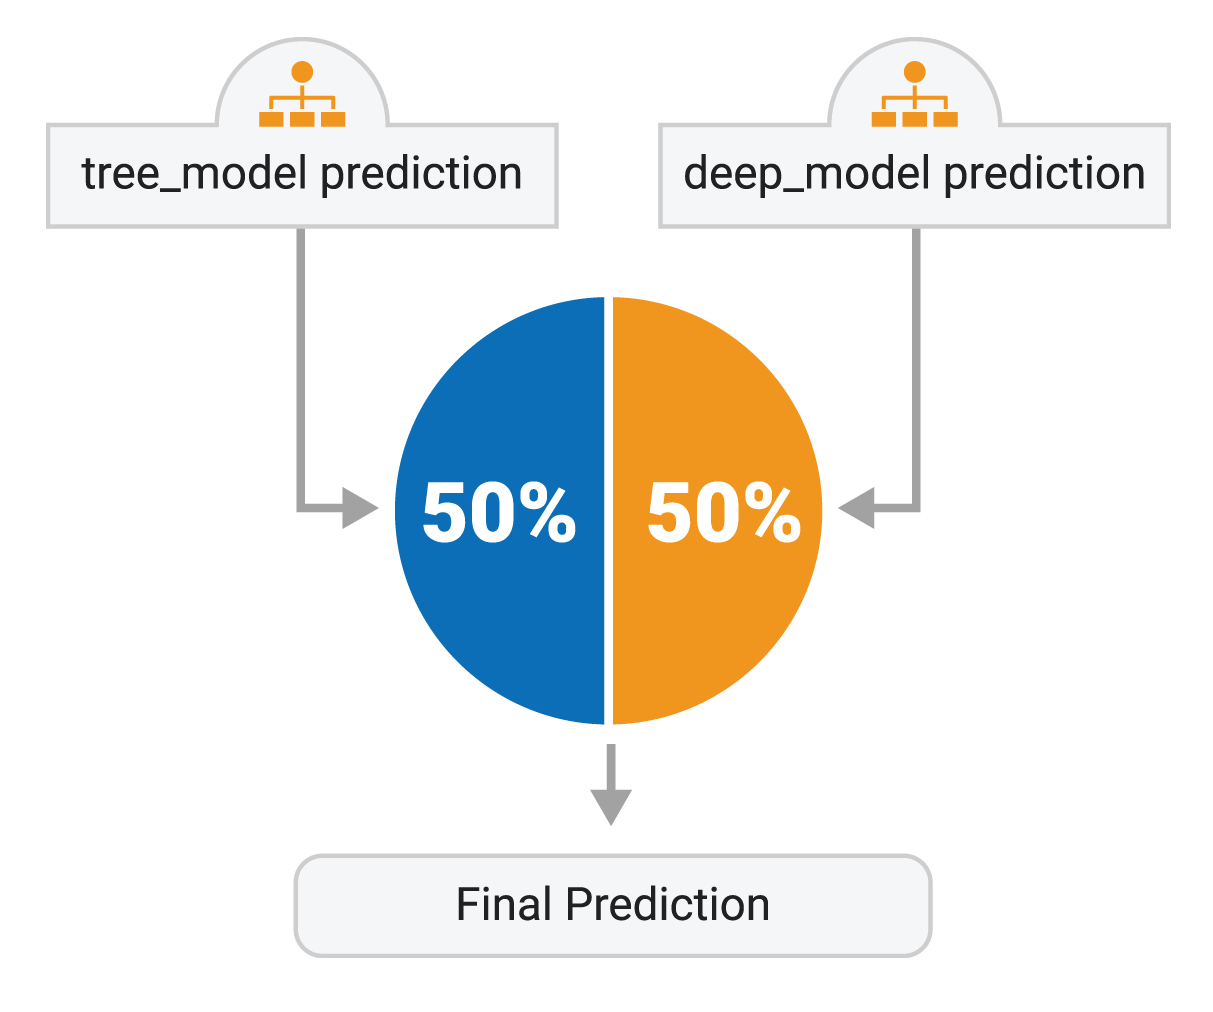
\includegraphics[scale=0.5]{../../img/model/solat_in_the_swen/final_prediction_light.png}
 \captionof{figure}{Modèle avec deux sous-modèles concurents de Talos.}
 \label{fig0}
\end{center}

L'équipe de Solat in the swen a implémenté plusieurs modèles performants.
Ils ont ensuite décidé de faire un modèle utilisant des systèmes concurants.
% Traits et modèles utilisés
Les traits entre la solutions de Talos et la baseline de la FNC ne changent pas.
Ils utilisent le même preprocessing et la même vectorisation.
Le modèle est composé de plusieurs systèmes concurents: le premier est un \textit{deep convolutional neural network} et le second est un \textit{gradient-boosted decision trees}.
%Algorithmes utilisés

Détaillons ici les algorithmes du modèles:
\begin{center}
 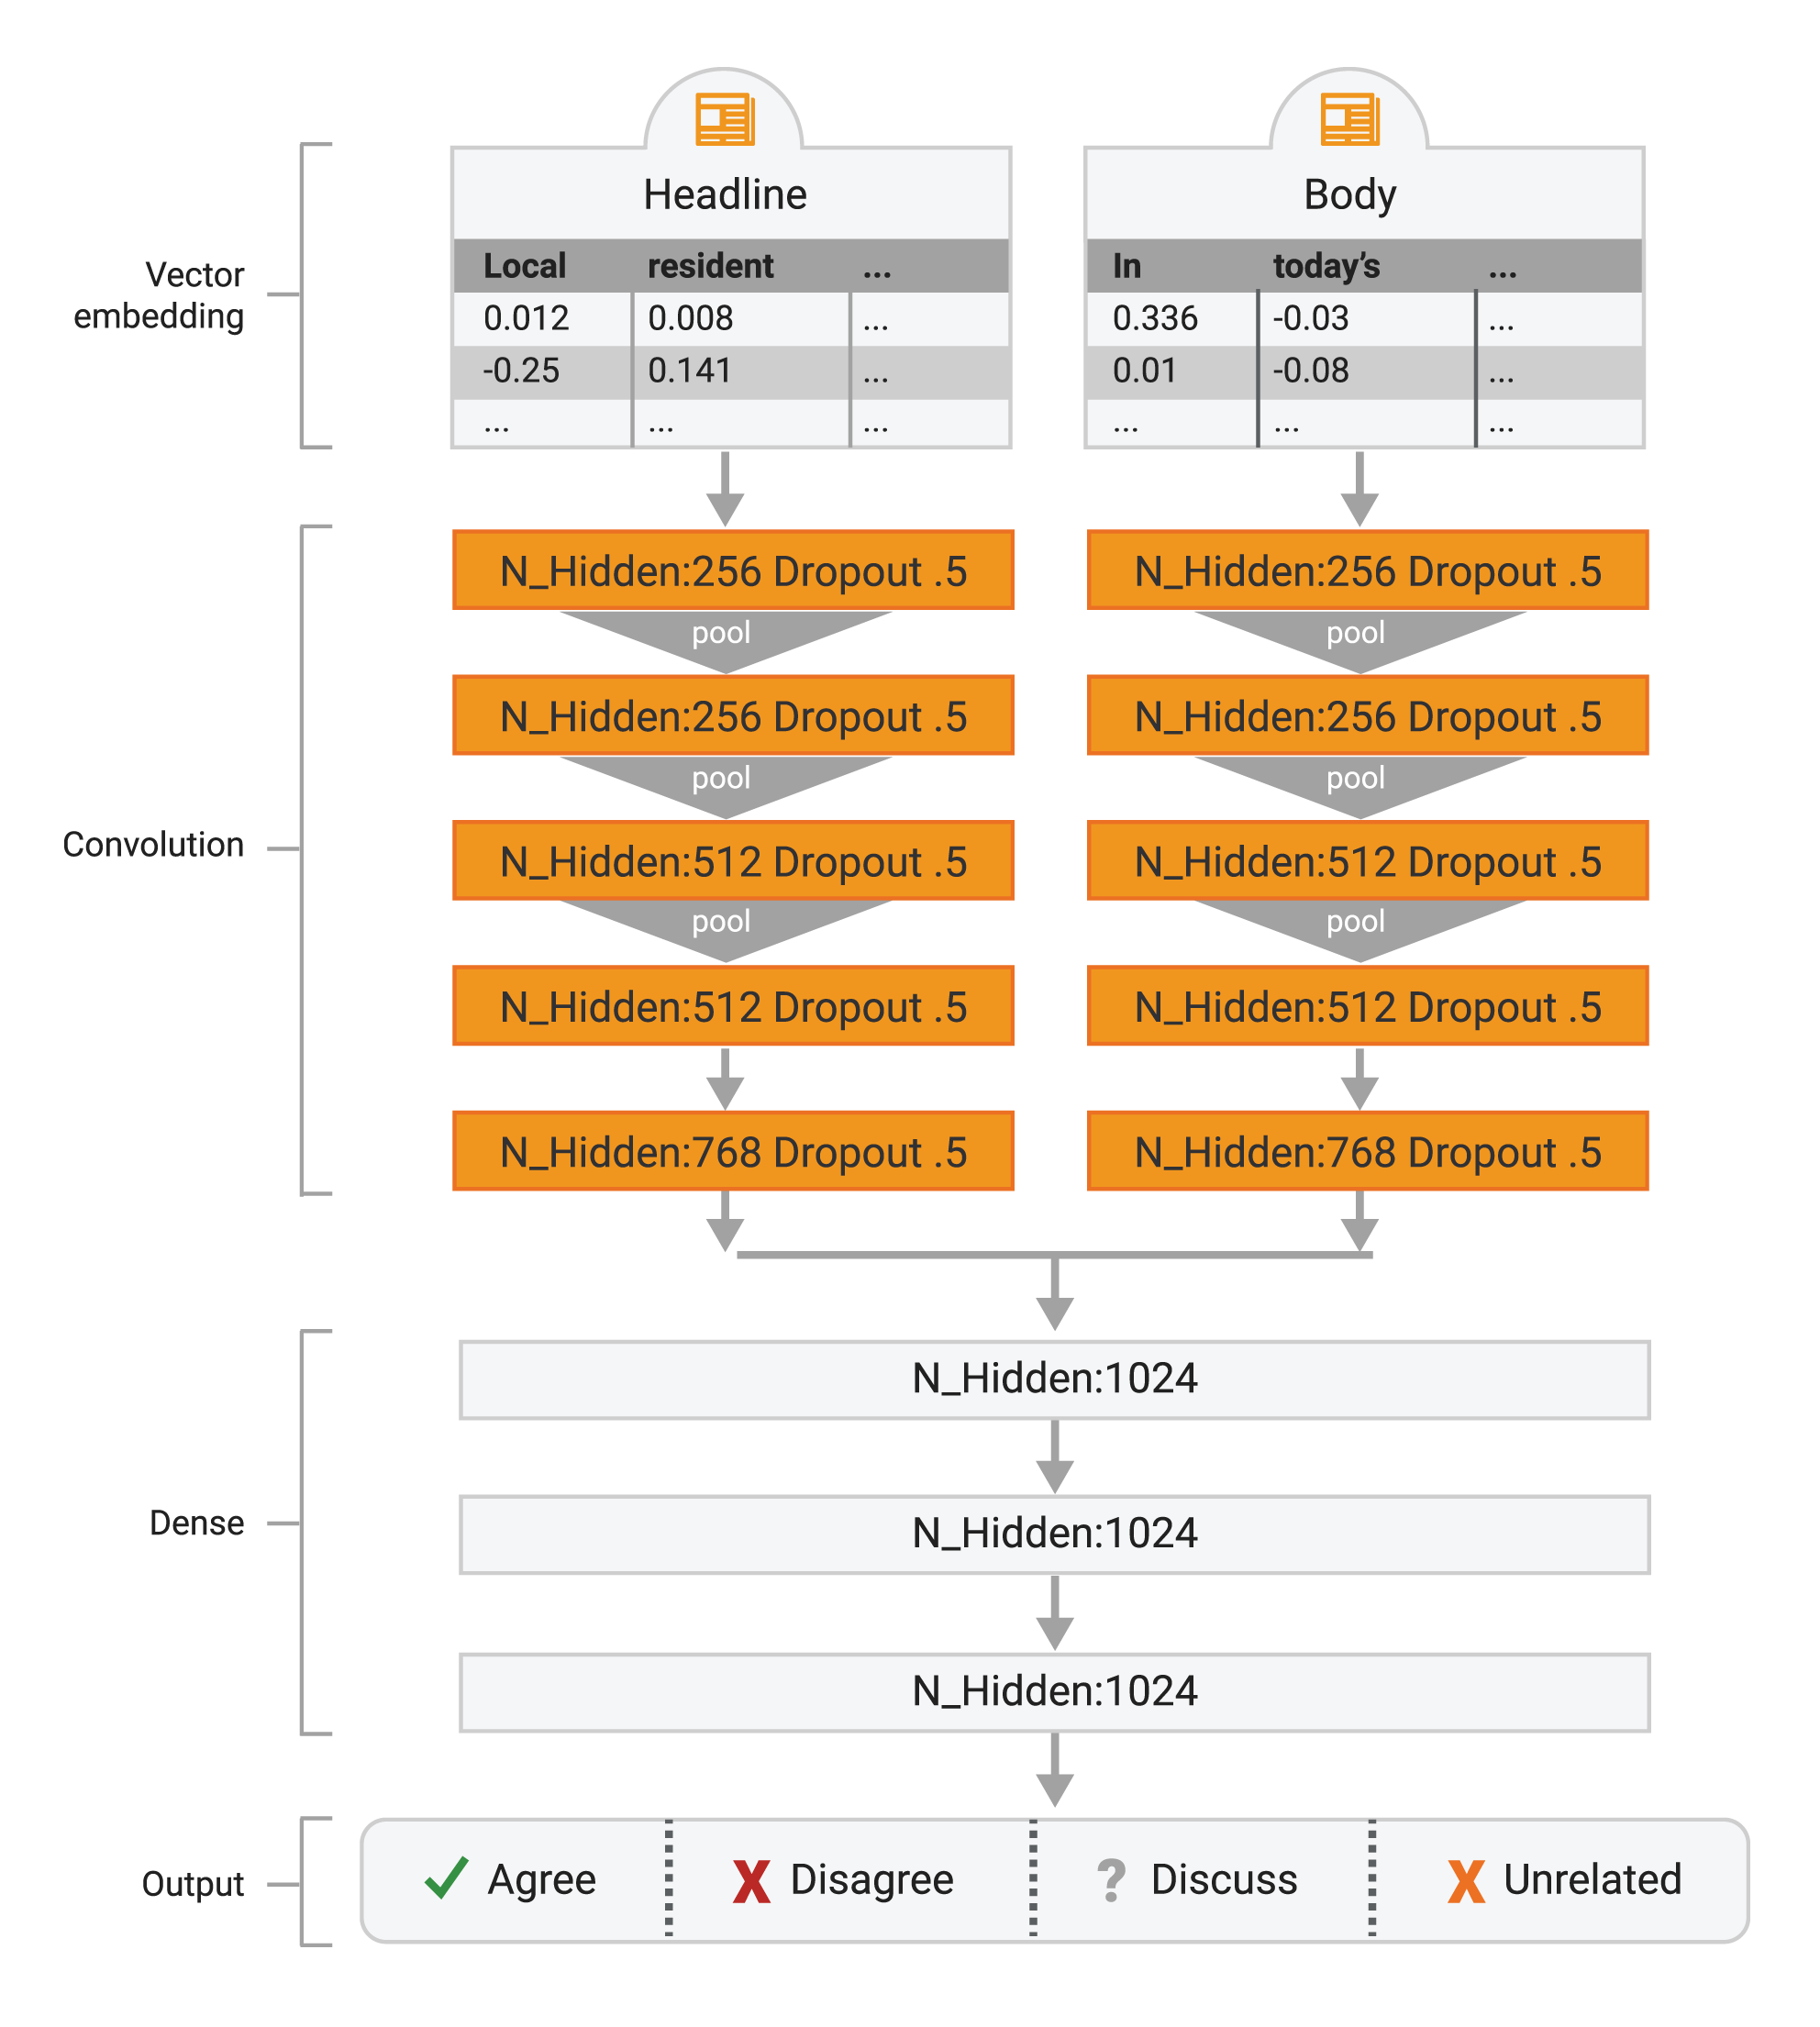
\includegraphics[scale=0.5]{../../img/model/solat_in_the_swen/deep_model_light.png}
 \captionof{figure}{Approche d'apprentissage en profondeur; modèle CNN + MLP.}
 \label{fig1}
\end{center}

Le premier modèle utilisé par l'équipe a plusieurs réseaux de neurones différents utilisés dans l'apprentissage en profondeur.
Ce modèle s'applique à la convolution numérique nette unidimensionnelle (CNN) sur le titre et le corps du texte, en utilisant les vecteurs préchargés de Google News.
Les CNN permettent un calcul parallèle efficace lors de l'exécution.
La sortie de ce CNN est ensuite envoyée à  MLP avec une sortie 4 classes:\og agree\fg, \og disagree\fg, \og discuss\fg et \og unrelated \fg, formés de bout en bout.
Cette architecture de ce modèle fut choisie en raison de sa facilité de mise en œuvre et de son calcul rapide puisque l'on peut compter sur des convolutions au lieu de récurrence.
Il est par contre limité par le fait qu'il ne peut observer le texte qu'une seule fois.


\begin{center}
 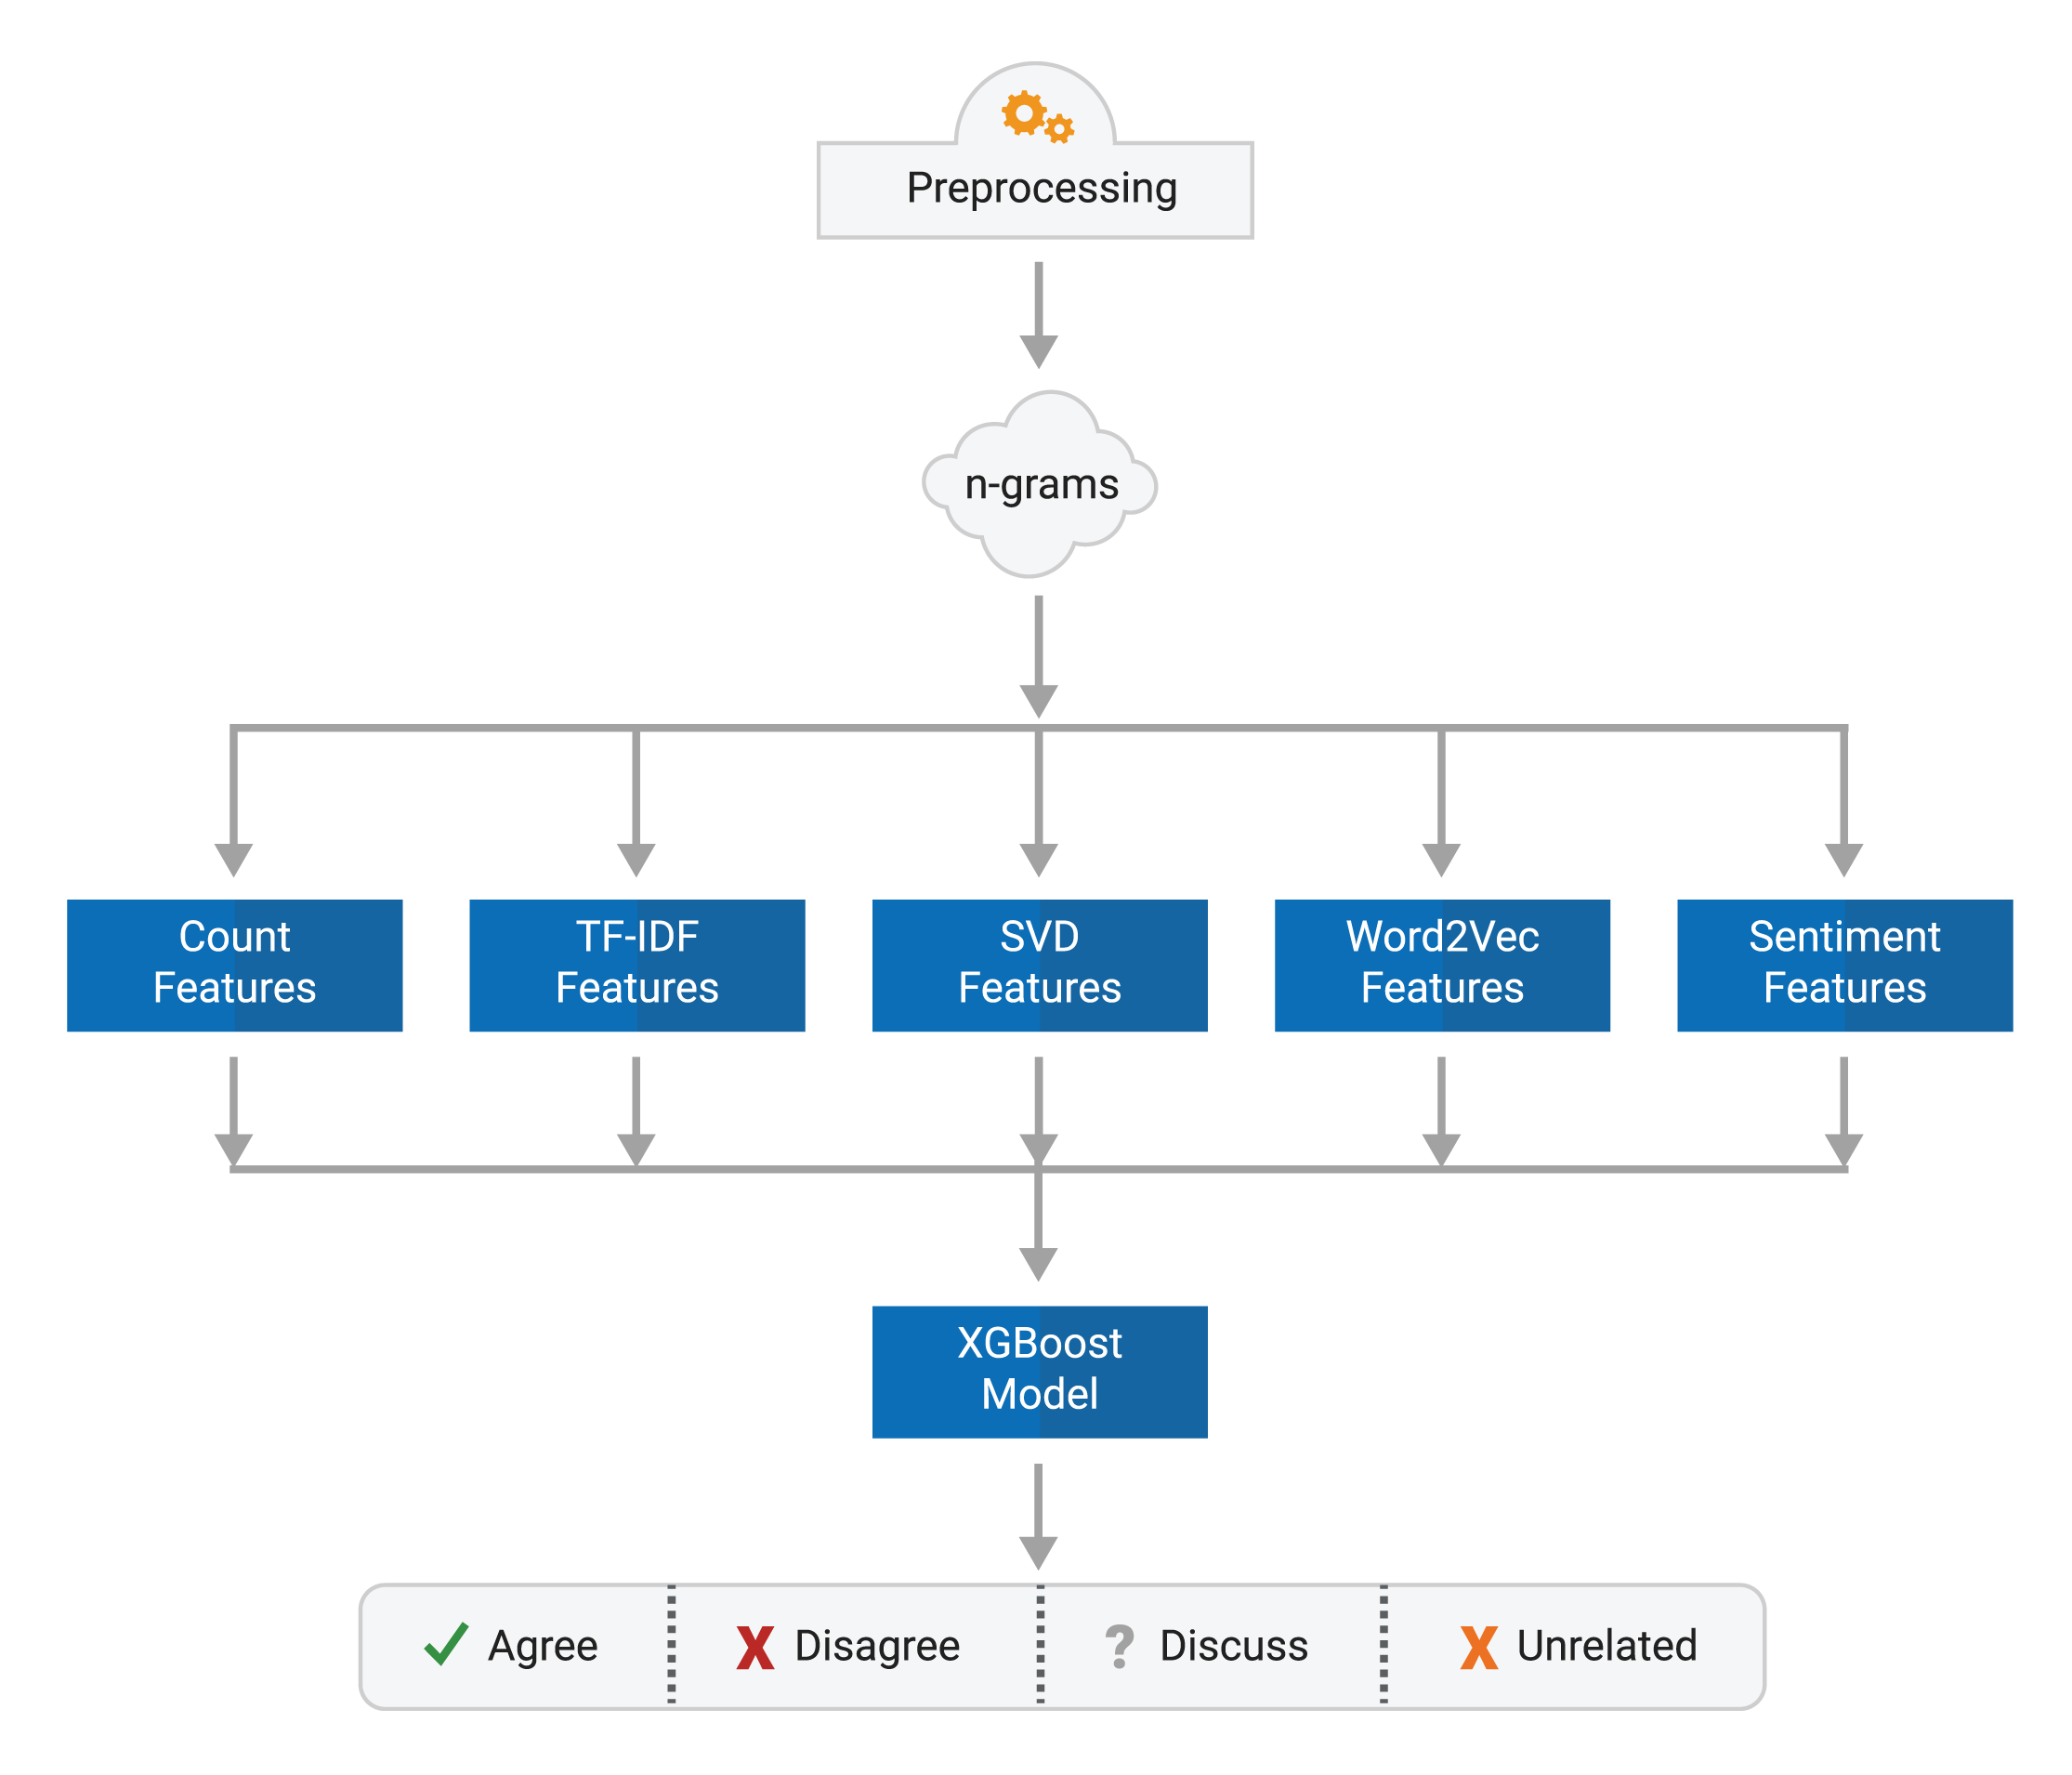
\includegraphics[scale=0.5]{../../img/model/solat_in_the_swen/tree_model_light.png}
 \captionof{figure}{Approche Gradient-Boosted Decision Trees}
 \label{fig2}
\end{center}

L'autre modèle utilisé dans l'ensemble est un modèle d'arbres de décision à gradient d'intensité (GBDT).
Ce modèle introduit peu de caractéristiques textuelles de l'affirmation de rumeurs et du corps de l'article, qui sont ensuite introduites dans le sujet d'un gradient dans la relation entre \textbf{C} et \textbf{E}. Ce modèle basé sur le texte entrainé avec XGBoost utilise plusieurs modules de décision à savoir:
\begin{description}
 \item [Un compteur de trait] pour compter le nombre de trait commun entre le titre et le corps de l'article.
 \item [La méthode de pondération TF-IDF] pour comparer de manière inversé la fréquence relative des mots.
 \item [Le procédé algebrique linéaire SVD Features] pour mesurer la similarité entre différents n-grams.
 \item [L'espace vectoriel word2vec] pour comparer le cosinus de similarité entre deux représentation vectorielle.
 \item [Un module Sentiment] utilisant un corpus de mots connotés sentimentalement.
 
\end{description}
Un \textbf{compteur de trait}, pour compter le nombre de trait commun entre le titre et le corps de l'article, la méthode de pondération \textbf{TF-IDF}; pour comparer de manière inversé la fréquence relative des mots, le procédé algebrique linéaire \textbf{SVD Features} pour mesurer la similarité entre différents n-grams, l'espace vectoriel \textbf{word2vec}; pour comparer le cosinus de similarité entre deux représentation vectorielle et un \textbf{module Sentiment} utilisant un corpus de mots connotés sentimentalement.

Les arbres de décision à gradient ont été choisis en raison de la robustesse du modèle par rapport aux différentes échelles des vecteurs caractéristiques.

\subsubsection{Résultats.}
Talos in the swen gagne le FNC avec une score de 9556.50 points donc un score relatif de 82.02\%.


%########################################################################################
%###########Athene (UKP Lab)#############################################################
%########################################################################################


\subsection{Athene (UKP Lab).}
\subsubsection{Méthodologie.}

\begin{center}
 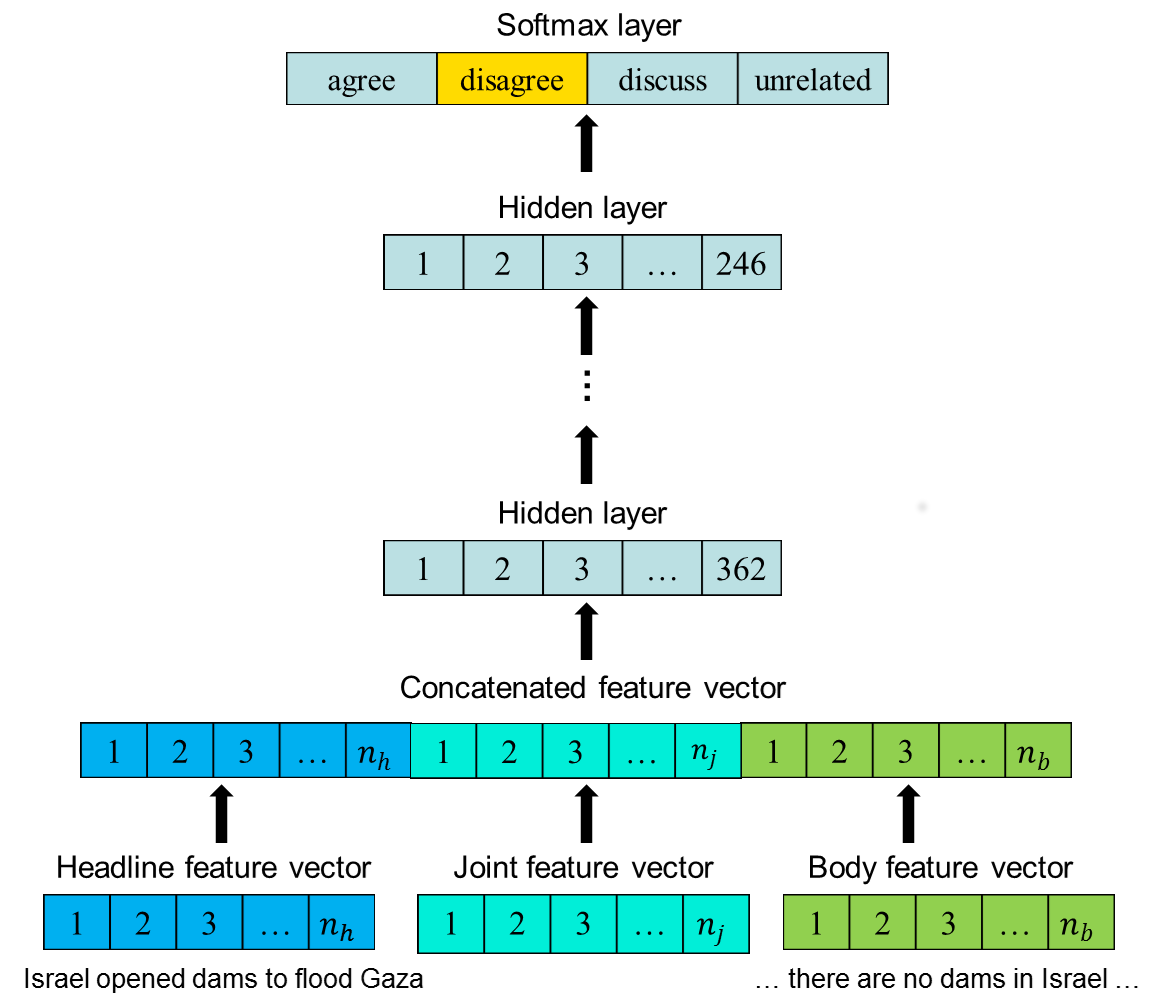
\includegraphics[scale=0.25]{../../img/model/athene/athene_model.png}
 \captionof{figure}{MLP utilisé pour FNC par l'équipe Athene}
 \label{fig3}
\end{center}

Le MLP proposé par Richard Davis et Chris Proctor (organisateurs de FNC) a été le point de départ pour le développement du
système final d'Athene.
La structure du système a été optimisée pour les
caractéristiques par une recherche aléatoire par laquelle les hyper-paramètres ont
été ajusté.
La structure du modèle qui en résulte est illustrée ci-dessus en résumé, car 5 des 7 couches cachées sont ignorées.

Le preprocessing d'Athene utilise différents traits, à savoir: les Bag of Words sur les uni-grams, les matrices de factorisations non-négatives, l'indexation et l'analyses latente sémantique (LSA, LSI) et la détection de paraphrase basé sur le recouvrement de mots (avec word2vec).

La vectorisation des informations se passe en trois étape la vectorisation des données préprocessées de \textbf{C} puis de \textbf{E} et la création d'un vecteur joint des dimension se recoupant dans les deux précédents vecteurs.
Ces trois vecteurs sont alors concaténés en un seul pour former une entrée.

Le modèle final rassemble cinq MLP initialisés de manière aléatoire, qui donnent leurs sorties à un seul MLP qui va faire le vote de la classes à attribuer à partir des autres MLP.
\subsubsection{Résultats}
Athene arrive deuxième au classement du FNC avec une score de 9550.75 points donc un score relatif de 81.97\%.

%########################################################################################
%###########UCL Machine reading##########################################################
%########################################################################################

\subsection{UCL Machine reading.}
\subsubsection{Méthodologie.}
\begin{center}
 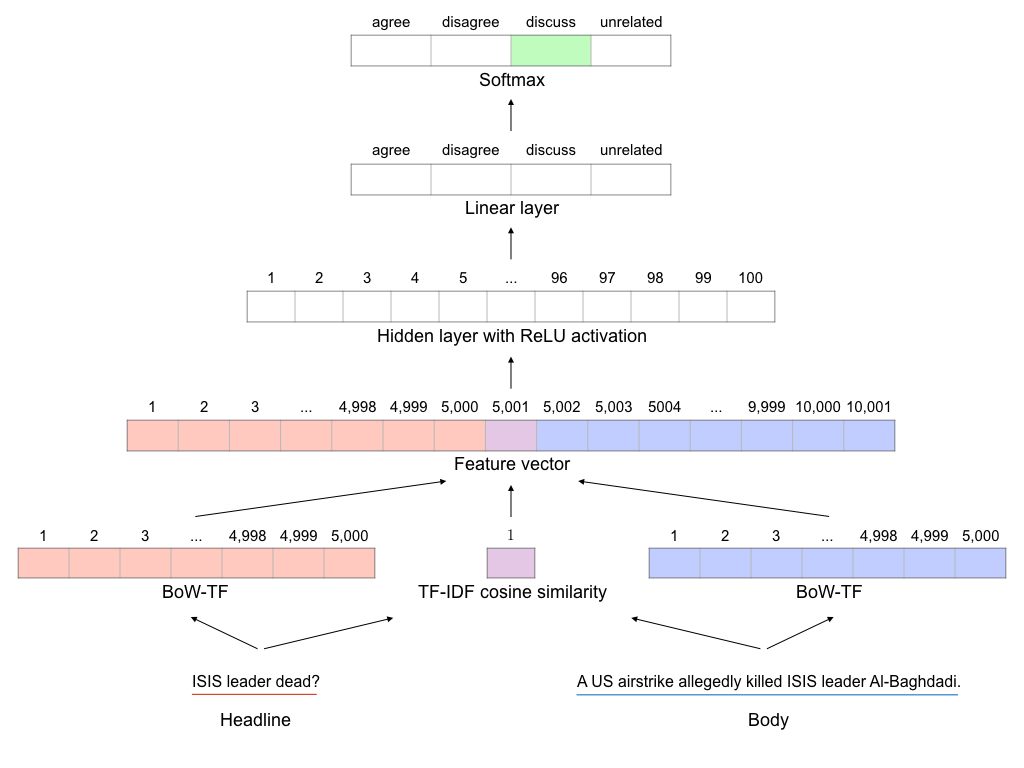
\includegraphics[scale=0.35]{../../img/model/uclmr/uclmr_model.png}
 \captionof{figure}{Schéma du modèle de l'UCLMR.}
 \label{fig4}
\end{center}
UCL-MR est juste un MLP (plutot simple par rapport aux autres solutions) entrainé sur les unigrams et une utilisation astucieuse du TF-IDF.

UCL utilise deux représentations simples des mots avec BoW pour les entrées de texte: fréquence de terme (TF) pour représenter l'affirmation \textbf{C} et le corps de l'article \textbf{E} et l'inverse de la fréquence de la fréquence du document (TF-IDF) pour calculer le cosinus de similarité entre \textbf{E} et \textbf{C}.

Ainsi les vecteurs d'entrée contiennent ces trois vecteurs composites.
Les vecteurs passent dans une seule couche d'entrée de 100 perceptrons avec une activation ReLU.
Puis une couche linear pour donner une valeur à chacune des classes.
Puis un softmax pour sortir la classe dominante.

UCL-MR utilise juste un MLP mais avec des paramètres très optimisés.
Nous ne détaillerons pas ici les paramètres d'implémentation qui se retrouvent dans leur publication.
\subsubsection{Résultats.}
UCL-MR arrive troisième au classement du FNC avec une score de 9521.50 points donc un score relatif de 81.72\%.

\subsection{Discussion comparative des modèles et des résultats.}
% tableau de comparaison des score
\begin{center}
 \begin{tabular}{| c || c | c | }
  \hline
  \textbf{Équipes} & \textbf{Scores bruts} & \textbf{Scores relatifs} \\
  \hline
  Talos in the Swen & 9556.50               & 82.02\%                  \\
  Athene            & 9550.75               & 81.97\%                  \\
  UCLMR             & 9521.50               & 81.72\%                  \\
  \hline
 \end{tabular}
 \captionof{table}{Résultats ordonnés de la FNC.}
\end{center}

Comme l'a dit Dean Domerleau (organisateur) en parlant de ce tableau de résultats: \og Ce que tout cela signifie, c'est que les meilleures équipes se sont très bien débrouillées, mais il y a certainement encore place pour l'amélioration!\fg.
En effet on pourrait pousser plus loin les sytèmes pour que ceux-ci nous donnent de meilleurs résultats.
Mais qu'il n'y ait pas de percée d'une équipe dans le tableau des scores, et le fait que très peu d'équipes on fait mieux que la baseline, montrent que cette tâche est difficile.

De plus un système complexe comme celui de Talos sensé être explicatif sur les traits pertinents ne se démarque que de 0,3 points du système d'UCLMR très peu explicatif mais bien otpimisé, qui reste une boîte noire au niveau de la sélection des paramètres.
On revient à un modèle régréssif qui est simple et qui explique beaucoup avec peu.
Mais cela donne une compréhension minime du phènomène.
Ou peut être le système d'UCLMR est surévalué pour cette ensemble de données.
En ce qui concerne Athene les résultats sont sensiblement les mêmes que Talos.
La complexité de leur modèle est aussi fait à partir d'apprentissages automatisés, certes moins complexe que Talos mais qui reste quand même un modèle avec des systèmes concurents.

Ce qu'il faudrait faire, c'est de comparer les outputs de chaque système et voir comment ils trient les classes \textbf{related}.
Ainsi on pourait faire des recoupements sur les données.
Cela permettrait de constater ce que les différents systèmes font à l'identique et ce qu'ils font différemments.
On en déterminerait les traits et les architectures de modèle relatifs aux classes de données.

C'est ce que je me propose de faire dans la première section de la partie 3 de ce mémoire.
Dans le but ensuite d'apporter une contribution originale à ce problème en partant des systèmes déjà réalisés.

\end{document}
\grid
